% Copyright 2007 by Till Tantau
%
% This file may be distributed and/or modified
%
% 1. under the LaTeX Project Public License and/or
% 2. under the GNU Public License.
%
% See the file doc/licenses/LICENSE for more details.

\documentclass[portuguese,10pt,xcolor=table]{bredelebeamer}
\setbeameroption{show notes}

\usepackage[brazil]{babel}
\usepackage[utf8]{inputenc}
\usepackage{times}
\usepackage{varwidth}
\usepackage{listings} % Código de programas
\usepackage{tikz}
\usepackage{pifont}
\usepackage[tikz]{bclogo}
\usepackage{tikzsymbols}
\usetikzlibrary{arrows,shapes}

\usetikzlibrary{calc,decorations.pathmorphing,patterns}
\pgfdeclaredecoration{penciline}{initial}{
	\state{initial}[width=+\pgfdecoratedinputsegmentremainingdistance,
		auto corner on length=1mm,]{
			\pgfpathcurveto%
			{% From
				\pgfqpoint{\pgfdecoratedinputsegmentremainingdistance}
				{\pgfdecorationsegmentamplitude}
			}
			{%  Control 1
				\pgfmathrand
					\pgfpointadd{\pgfqpoint{\pgfdecoratedinputsegmentremainingdistance}{0pt}}
				{\pgfqpoint{-\pgfdecorationsegmentaspect
							   \pgfdecoratedinputsegmentremainingdistance}%
							   {\pgfmathresult\pgfdecorationsegmentamplitude}
				}
			}
			{%TO 
				\pgfpointadd{\pgfpointdecoratedinputsegmentlast}{\pgfpoint{1pt}{1pt}}
			}
		}
	\state{final}{}
}



\everymath{\displaystyle}
\tikzstyle{every picture}+=[remember picture,decoration=penciline]
\DeclareTextFontCommand{\textdf}{\bfseries\color{blue!80}}
%\tikzstyle{every node}+=[decorate]
%\tikzstyle{every path}+=[decorate]
%\tikzstyle{na} = [baseline=-.5ex]

\usepackage[T1]{fontenc}

\def\lecturename{IMD0012 - Introdução às técnicas de programação}

\title{\insertlecture}
\author{Prof. Fernando Figueira\\(adaptado do material do Prof. Rafael Beserra Gomes}
\institute{UFRN}

\subject{Estruturas de Repetição}

\lecture[]{Estruturas de Repetição}{}

\date{}

\def\exe[#1]{\color{gray}#1\color{black}}
\def\exp[#1]{\color{gray}<\textit{#1}>\color{black}}
\def\espaco{\color{gray}\hspace{0.2cm}\color{black}}
\def\espaco{\color{blue}␣\color{black}}
\def\inativo[#1]{\color{gray}#1\color{black}}

\definecolor{deepgreen}{rgb}{0,0.5,0}
\lstset{
	language=C,
	basicstyle=\footnotesize\ttfamily,
	%basicstyle=\scriptsize\ttfamily,
	keywordstyle=\footnotesize\bfseries\sffamily,
	%keywordstyle=\scriptsize\bfseries\sffamily,
	showstringspaces=false,
	numbers=left,
	numberstyle=\footnotesize,
	stepnumber=1,
	numbersep=5pt,
	tabsize=4,
	%backgroundcolor=\color{blue!05},
	backgroundcolor=\color{gray!35},
	showspaces=false,
	showtabs=false,
	stringstyle=\ttfamily\color{red!80!brown},
	commentstyle=\ttfamily\color{blue!80},
	keywordstyle=\bfseries\color{deepgreen},
	escapeinside={\%*}{*)}
	}
	\renewcommand{\lstlistingname}{Código}
\begin{document}

\usebackgroundtemplate{%
	
\includegraphics[width=\paperwidth,height=\paperheight]{background2}
}
\begin{frame}
  \maketitle
 \begin{center}
 \tiny
Material compilado em \today.\\
  Licença desta apresentação:\\
		
\includegraphics[height=1.0cm]{by-nc-nd.png}\\
http://creativecommons.org/licenses/
	\end{center}
\end{frame}


	\def\GN[#1]{\colorbox{gray!40}{#1}}
	\def\RN[#1]{\colorbox{red!40}{#1}}
	\def\BN[#1]{\colorbox{blue!40}{#1}}
	\def\ON[#1]{\colorbox{orange!40}{#1}}
	\def\WN[#1]{\colorbox{white!40}{#1}}


\section{Estruturas de repetição}

	\begin{frame}[c]
		\begin{center}
			\structure{\large \insertsection}
		\end{center}
	\end{frame} 
	
	
	\begin{frame}
		\begin{itemize}
			\item Em determinados momentos queremos \textbf{repetir} uma mesma instrução ou um bloco de instruções por várias vezes
			\item Por exemplo: escrever na tela os números de 1 a 100
				\lstinputlisting{umacemA.c}
			\item Por que é inviável escrever o mesmo bloco de instruções diversas vezes?
		\end{itemize}
	\end{frame}	

	\begin{frame}
		\begin{itemize}
			\item Outro exemplo: quais os divisores de um número?
				\lstinputlisting{divisoresA.c}
			\item Você pode não saber quantas vezes repetir, pois o número de repetições pode ser em função de alguma variável
		\end{itemize}
	\end{frame}	
	
	
	\begin{frame}
        \begin{itemize}
            \item \textdf{Estrutura de repetição}: repetir um \textbf{bloco de instruções}
            \item \textdf{Iteração}: cada repetição
        \end{itemize}
		Veremos as seguintes estruturas de repetição:
		\begin{itemize}
		\item while
		\item do/while
		\item for
		\end{itemize}
        
	\end{frame}

\section{Estrutura while}

	\begin{frame}[c]
		\begin{center}
			\structure{\large Estrutura de repetição \textbf{while} (enquanto)}
		\end{center}
	\end{frame} 

    \begin{frame}
		\begin{columns}[t]
			\begin{column}[T]{.6\textwidth}
				while(\exp[expressão lógica]) \{\\
				\espaco \exp[instrução 1]\\
				\espaco \exp[instrução 2]\\
				\espaco \exp[...]\\
				\espaco \exp[instrução n]\\
				\}
			\end{column}
							\begin{column}[T]{.4\textwidth}
								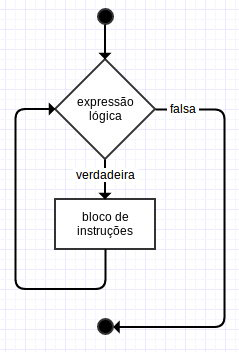
\includegraphics[height=5.0cm]{fluxogramaWhile.png}
							\end{column}
		\end{columns}
		\begin{itemize}
			\item o bloco de instruções é executado \textdf{enquanto} o valor da expressão lógica \textdf{for verdadeiro}
			\item bastante útil quando não sabemos o número de iterações
		\end{itemize}
	\end{frame}

    \begin{frame}
	    Exemplo: escrevendo os números de 1 a 100
			\lstinputlisting{umacemC.c}
		
	\end{frame}

    \begin{frame}
	    Exemplo: quais os divisores de um número?
			\lstinputlisting{divisoresC.c}
		
	\end{frame}
    
	\begin{frame}
		\bcattention \hspace{0.3cm} Cuidado com a \textdf{indentação}!!
			\lstinputlisting{divisoresD.c}
		
	\end{frame}
	
	\begin{frame}
	\begin{alertblock}{\ding{46} Exercício em sala}
		Escreva um programa em C que leia um número inteiro \textbf{n}. Depois o programa deve escrever na tela todos os números pares de 1 a \textbf{n} e depois todos os números ímpares de 1 a \textbf{n}.
		
		Exemplo:
		\colorbox{gray!15}{
			\begin{varwidth}{700px}
				Digite n: \textbf{8}\\
				Pares: 2 4 6 8\\
				Ímpares: 1 3 5 7
			\end{varwidth}
		}\\
	\end{alertblock}
	\end{frame}

	\begin{frame}
	\begin{alertblock}{\ding{46} Exercício em sala}
	    \textbf{Problema 3*n + 1}: dado um número n, se este número for par, divida-o por 2 e se for ímpar, multiplique por 3 e some 1. Repita o processo até chegar no número 1.
		
		Escreva um programa em C que leia um número inteiro \textbf{n} e escreva na tela a sequência gerada pelas regras acima.
		
		Exemplo:
		\colorbox{gray!15}{
			\begin{varwidth}{700px}
				Digite n: \textbf{5}\\
				5 16 8 4 2 1
			\end{varwidth}
		}\\
	\end{alertblock}
	\end{frame}


\section{Estrutura do/while}

	\begin{frame}[c]
		\begin{center}
			\structure{\large Estrutura de repetição \textbf{do/while} (faça/enquanto)}
		\end{center}
	\end{frame} 

    \begin{frame}
		\begin{columns}[t]
			\begin{column}[T]{.6\textwidth}
				do \{\\
				\espaco \exp[instrução 1]\\
				\espaco \exp[instrução 2]\\
				\espaco \exp[...]\\
				\espaco \exp[instrução n]\\
				\} while(\exp[expressão lógica]);
			\end{column}
							\begin{column}[T]{.4\textwidth}
								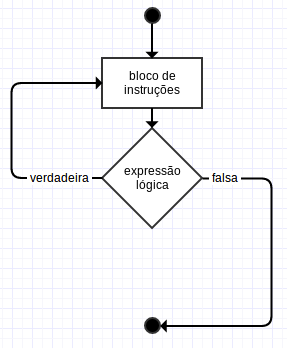
\includegraphics[height=5.0cm]{fluxogramaDoWhile.png}
							\end{column}
		\end{columns}
		\begin{itemize}
			\item o bloco de instruções é executado \textdf{e continua sendo executado} \textbf{enquanto} o valor da expressão lógica \textbf{for verdadeiro}
			\item use-o quando o bloco de instruções precede o primeiro teste
		\end{itemize}
	\end{frame}

    \begin{frame}
	    Exemplo: lê dois números a e b. O valor de b deve ser solicitado novamente enquanto for 0. Em seguida, escreve o resultado da divisão $\frac{a}{b}$.
			\lstinputlisting{entrada.c}
		
	\end{frame}


	\begin{frame}
	\begin{alertblock}{\ding{46} Exercício em sala}
	\textbf{Acerte a senha: } escreva um programa que leia um número inteiro. O programa deve prosseguir somente quando esse número for igual a uma senha que você definir no código. Escreva em seguida o número de tentativas para acertar a senha.
	\end{alertblock}
	\end{frame}


\section{Estrutura for}

	\begin{frame}[c]
		\begin{center}
			\structure{\large Estrutura de repetição \textbf{for} (para)}
		\end{center}
	\end{frame} 
	
	\begin{frame}
		\begin{columns}[t]
			\begin{column}[T]{.8\textwidth}
				for(\exp[inicialização] ; \exp[expressão lógica]; \exp[incremento]) \{\\
				\espaco \exp[instrução 1]\\
				\espaco \exp[instrução 2]\\
				\espaco \exp[...]\\
				\espaco \exp[instrução n]\\
				\}
			\end{column}
							\begin{column}[T]{.2\textwidth}
								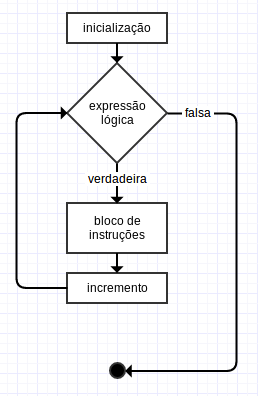
\includegraphics[height=4.0cm]{fluxogramaFor.png}
							\end{column}
		\end{columns}
		\begin{itemize}
			\item \textdf{inicialização}: executado antes da estrutura de repetição
			\item \textdf{expressão lógica}: avaliado antes de cada iteração (encerra caso falso)
			\item \textdf{incremento}: executado após cada iteração
		\end{itemize}
	\end{frame}

	\begin{frame}
	    Exemplo: escrevendo os números de 1 a 100
			\lstinputlisting{umacemB.c}
		
	\end{frame}

	\begin{frame}
	    Exemplo: quais os divisores de um número?
			\lstinputlisting{divisoresB.c}
		
	\end{frame}

	\begin{frame}
	\begin{alertblock}{\ding{46} Exercício em sala}
	Escreva um programa em C que leia um número inteiro \textbf{n} e escreva na tela se esse número é primo.
	\end{alertblock}
	\end{frame}


\section{For ou While?}

	\begin{frame}[c]
		\begin{center}
			\structure{\large Escolhendo entre for e while}
		\end{center}
	\end{frame} 
	\begin{frame}
		\begin{itemize}
			\item \textbf{reflita} como o uso de uma ou outra estrutura de repetição pode afetar a legibilidade do código
								\lstinputlisting{estranho.c}
		\end{itemize}
		
	\end{frame}
	\begin{frame}
		\begin{itemize}
			\item no geral:
			\begin{itemize}
			\item \textdf{for}: aplicada principalmente para percorrer um intervalo numérico\\
								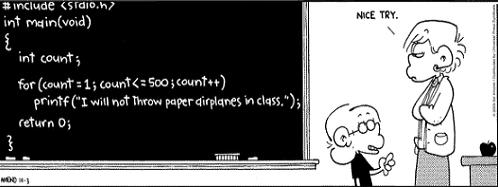
\includegraphics[height=3.5cm]{lousa.jpg}
			\item \textdf{while}: aplicada principalmente quando o número de iterações é desconhecido
		\end{itemize}
		\end{itemize}
		
	\end{frame}

\end{document}

